% VLDB template version of 2020-08-03 enhances the ACM template, version 1.7.0:
% https://www.acm.org/publications/proceedings-template
% The ACM Latex guide provides further information about the ACM template

\documentclass[sigconf, nonacm]{../tex_template/acmart}

%% The following content must be adapted for the final version
% paper-specific
\newcommand\vldbdoi{XX.XX/XXX.XX}
\newcommand\vldbpages{XXX-XXX}
% issue-specific
\newcommand\vldbvolume{14}
\newcommand\vldbissue{1}
\newcommand\vldbyear{2020}
% should be fine as it is
\newcommand\vldbauthors{\authors}
\newcommand\vldbtitle{\shorttitle} 
% leave empty if no availability url should be set
\newcommand\vldbavailabilityurl{http://vldb.org/pvldb/format_vol14.html}
% whether page numbers should be shown or not, use 'plain' for review versions, 'empty' for camera ready
\newcommand\vldbpagestyle{plain} 

\usepackage{makecell}
\usepackage{flexisym}
\usepackage{mathtools}
\DeclarePairedDelimiter\norm{\lVert}{\rVert}
\usepackage{fancyhdr}

\begin{document}
\title{COEN6311 Deliverable 1: Software Specification GroupSuper}

%%
%% The "author" command and its associated commands are used to define the authors and their affiliations.
\author{Ding Li 40160073, Zerui Wang 40177315, Jun Huang 40168167}

\maketitle

\section{Introduction}
\textbf{Brief of the system}

We define a system named \textbf{ICDE-ScholarHub} which is a web-based Paper Search Engine with ICDE concepts implemented.

The system will practice the idea of ICDE to help the researchers work more efficiently regarding user operation history, teamwork, and paper trending.

Furthermore, the system exposes the API of ICDE for the development of 3rd-party applications or plugins.

\section{Problem Statement}
\textbf{Describtion of the general problem that the system aims to solve.}

During the daily research work, it always happens that researchers forget some critical paper they have read on the web-based paper search system a long-time ago. It takes time to find the critical one from the huge amount of paper list from a different academic area.

More sadly, people may miss the latest paper which is important to their research. Researchers have supervisors, colleagues, and teammates. They like to share the latest paper in the same area with the team. But they do not want to disturb others by sending papers through email too often and it is not well organized.

If there is a  system that implements ICDE API, the reading history will be well recorded. The system will log down every activity the user performed.

For example, the researcher can develop a small tool to log down his paper reading history; the research team can develop a tool for sharing team member’s paper reading history,  paper marking history, area preference, and so on.

The aim of using ICDE-ScholarHub on the paper search system is to help the researchers and their teams work in a more efficient way.



\section{System architecture}
\textbf{Concrete context (architecture) of the system}

As shown in the Figure \refeq{fig:arch}, users can access the system through the system website on the browser over the network.

The system should implement ICDE API for the capture of user operation data and the access of those data. ICDE API should expose to the 3rd-party developer.

In particular, the system should have two databases. One for the main functions of Paper Search, one for user activities data.

\section{Project Goal}
\textbf{Key functionalities of and use cases of the system}

\subsection{Key functionalities}

The key functionalities are paper heading history record,
It would be good if there is software which can show the papers your colleagues are reading. Such as, what have they read before? Which area is their interest and which paper is worth a “like'' and “dislike”. How many hours they spent on this paper. Who may need to have a look at this paper? The paper which received many “likes” could be recorded and pushed to the relevant researcher in the lab.

Our ICDE APP should have two top modules described as Figure \refeq{fig:uc}.

\begin{figure*}[htp]
	\centering
	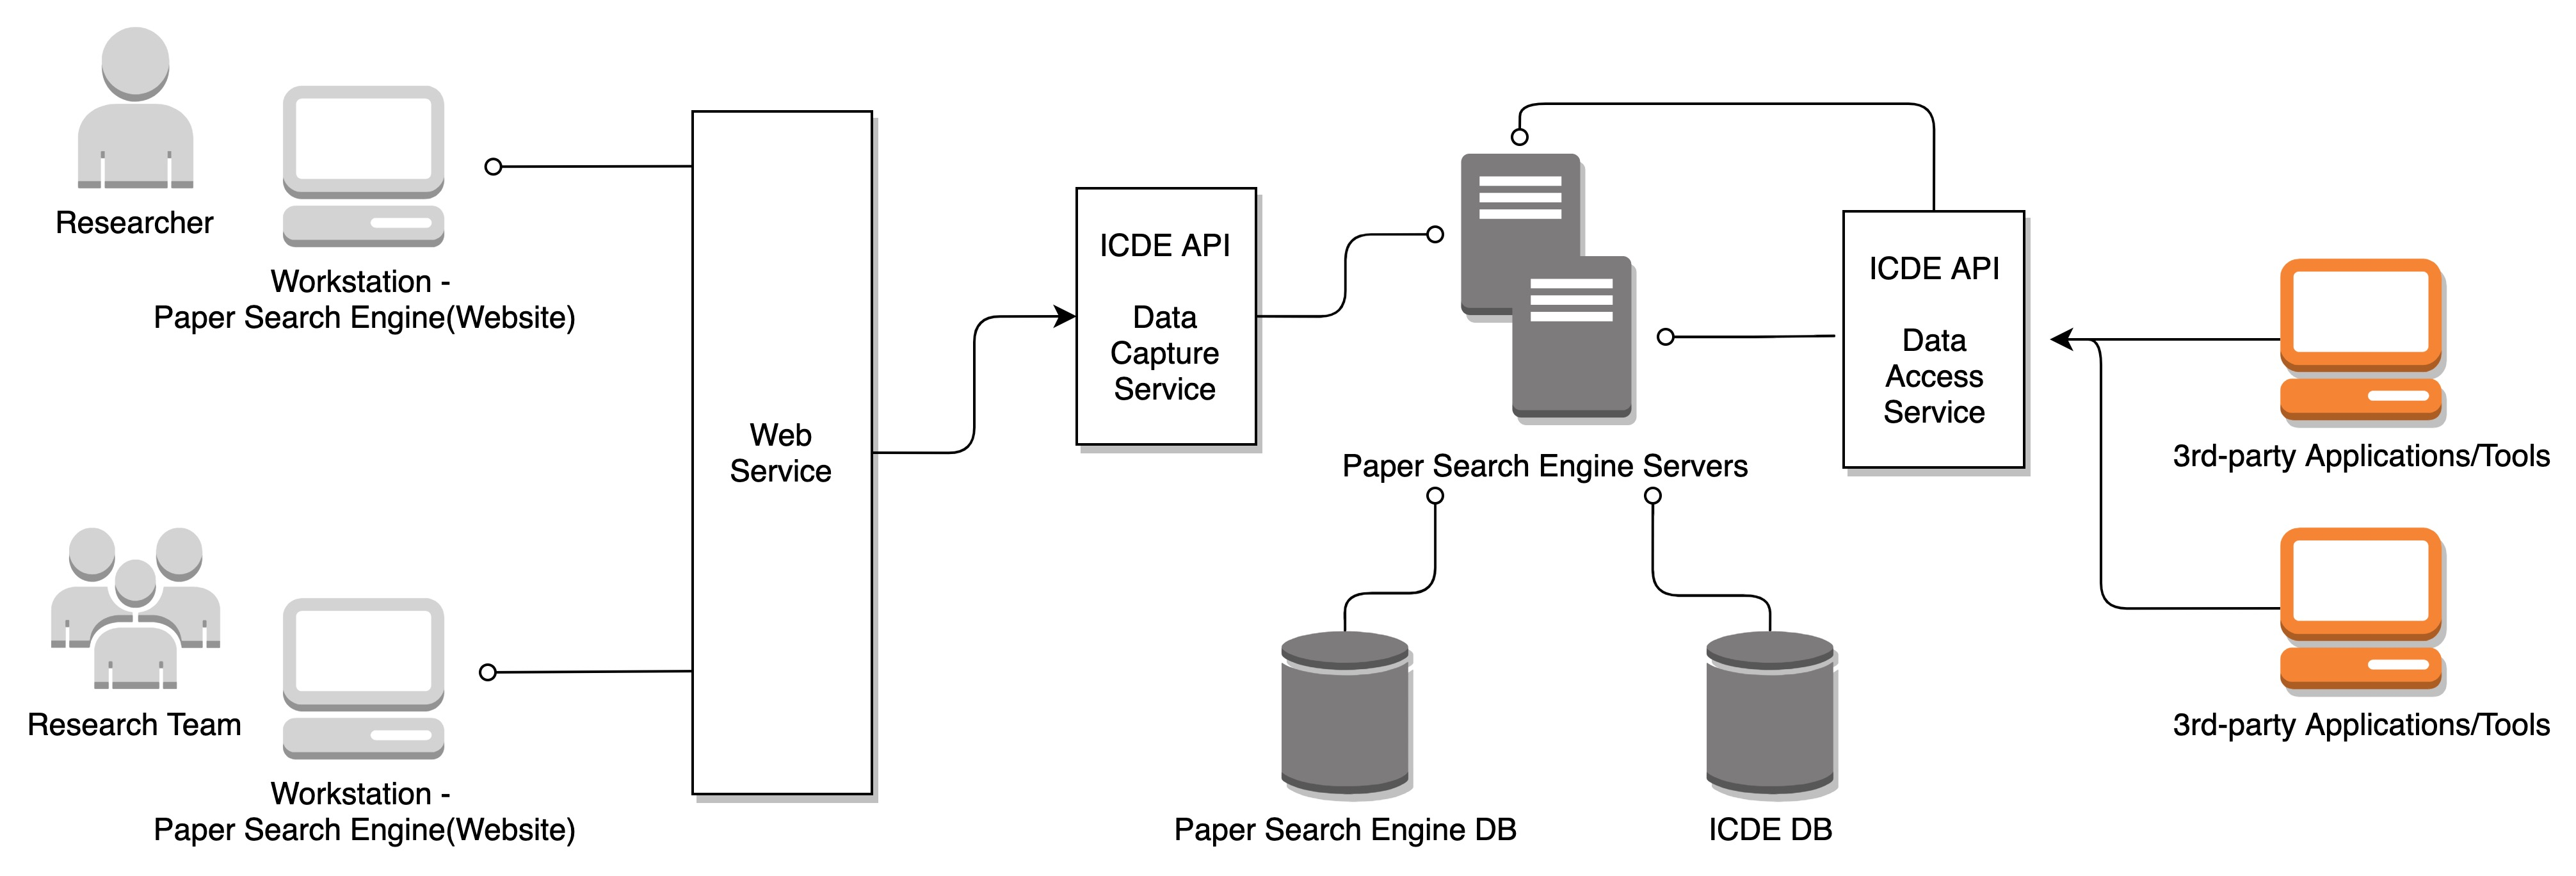
\includegraphics[scale=0.1]{D1F1.png}
	\caption{Architecture of ICDE-ScholarHub}
	\label{fig:arch}
\end{figure*}

\textbf{Key functions/sub-modules for PaperSearchEngine module:}

\begin{itemize}
	\item [1)]
	      User Information Management;
	\item [2)]
	      Paper Management;
	\item [3)]
	      Paper Searching Module;
\end{itemize}

\textbf{Key functions for ICDE module:}

\begin{itemize}
	\item [1)]
	      Capture users’ paper-relevant activities on the website;
	\item [2)]
	      Store \& organize those activities as records;
	\item [3)]
	      Expose API for accessing those records;
\end{itemize}

\subsection{Use cases}

A concrete Use Cases Diagram has shown below in Figure \refeq{fig:uc}

\begin{figure*}[htp]
	\centering
	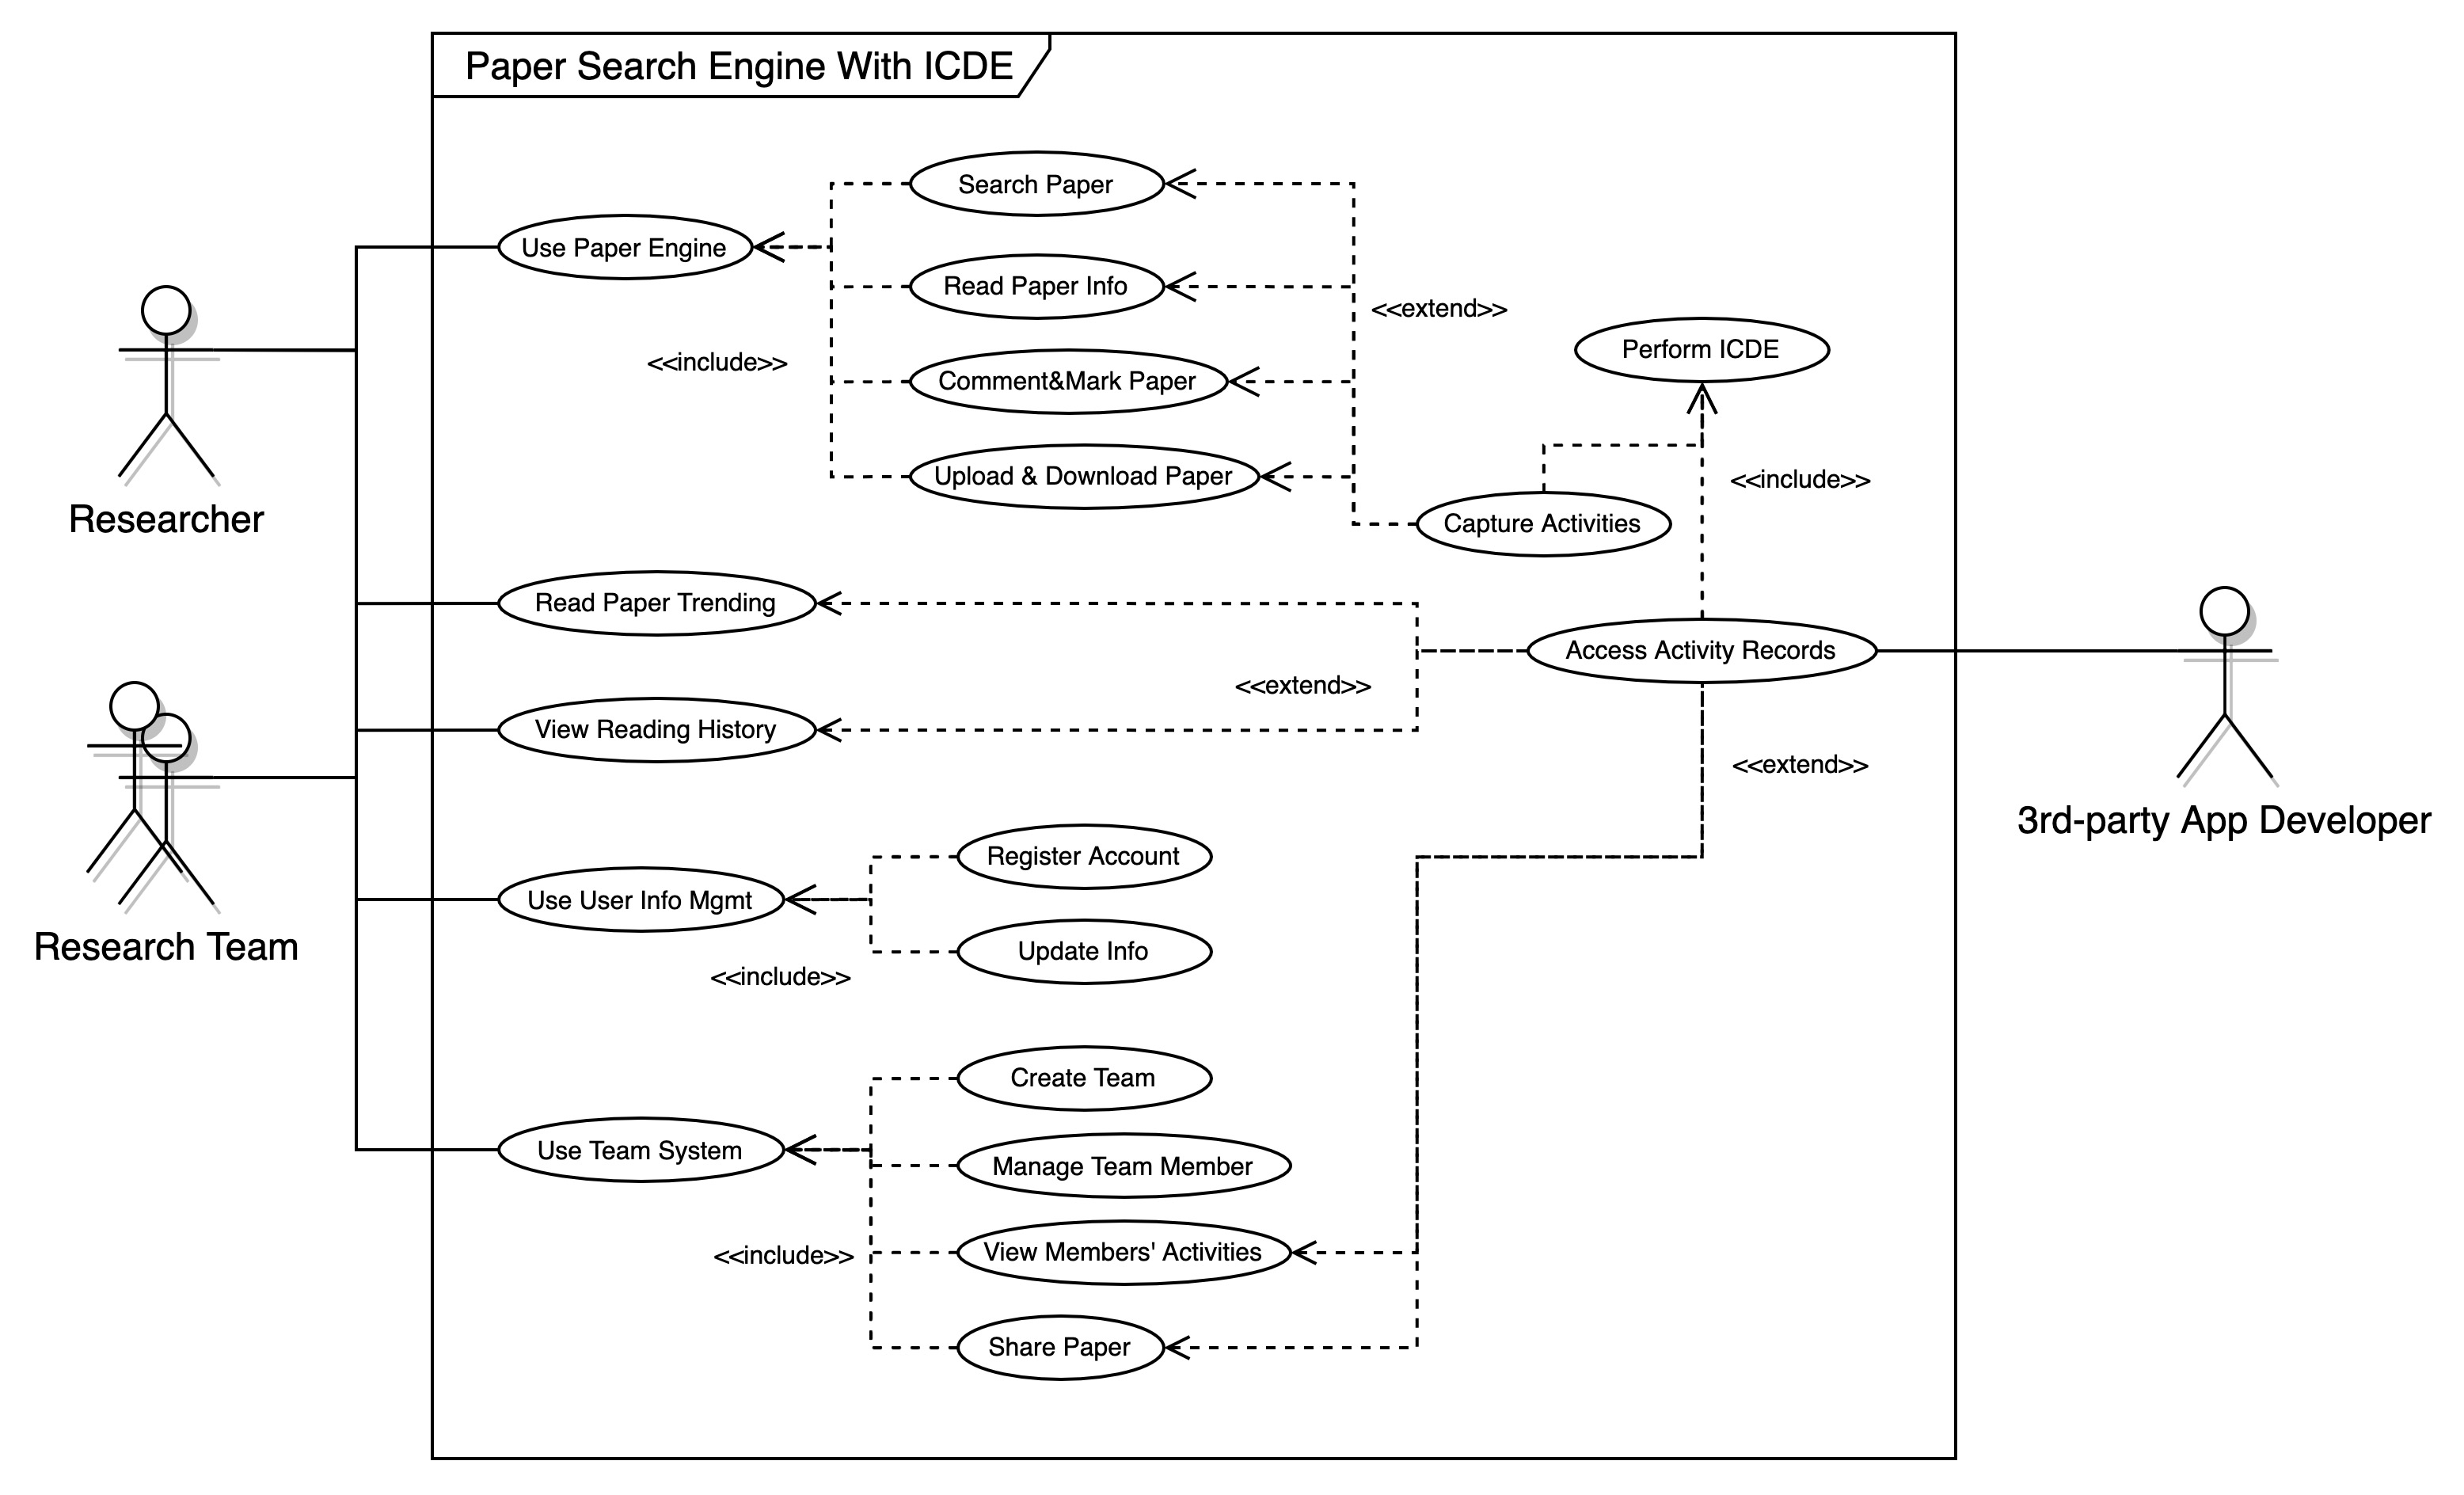
\includegraphics[scale=0.13]{D1F2.png}
	\caption{Use cases}
	\label{fig:uc}
\end{figure*}

\section{System User Stories}
\textbf{Describe “user stories” for each use case}

Table \refeq{table:1}, table \refeq{table:2} and table \refeq{table:3} are presenting three user stories for better understanding of the system.

\begin{table}[h!]
	\begin{tabular}{ l }
		\hline
		\textbf{Story 1: Researcher}                                  \\
		\hline
		Jack is a new university student. He got an individual        \\
		assignment last week from one of the courses which require    \\
		academic research. With the assignment demand, Jack should    \\
		search at least 3 to 4 academic papers for investigation.     \\
		So he heads to the \textbf{ICDE-ScholarHub} website.          \\
		\\
		He goes to the website and registers an account of it by      \\
		filling in all the information required by the website.       \\
		\\
		After finished registering, he then type some keywords of     \\
		the subject from the assignment. The website displays all     \\
		the results that match the keywords.                          \\
		\\
		He can read some information about the paper on its detail    \\
		page. He will know the authors, the year of the publication,  \\
		the academic area, and the abstraction. He will know that     \\
		how many people are like this paper, what are the comments    \\
		of it.                                                        \\
		\\
		Then he clicks the "download" button and then gets the pdf    \\
		file of this paper.                                           \\
		\\
		After finish the reading of it, he then login to the website, \\
		writes a comment about it and clicks the "dislike" button to  \\
		express his idea of this paper.                               \\
		\hline
	\end{tabular}
	\caption{A new user's story}
	\label{table:1}
\end{table}

\begin{table}[h!]
	\begin{tabular}{ l }
		\hline
		\textbf{Story 2: Researcher}                                   \\
		\hline
		Lucy is a Ph.D. student researching a program for several      \\
		months. She likes to use the system for paper searching.       \\
		\\
		After work, she will check the paper trending list once to     \\
		twice a season. With this trending list, it is easy to notice  \\
		what are the most popular topics and papers people like during \\
		the past season.                                               \\
		\\
		She will know how many people have visited the detail page     \\
		of the paper. She will know how many new "like" have been      \\
		given for the paper from other users.                          \\
		\\
		And when she is at work, she can see her paper browsing        \\
		history on the website and then find the one she wants to      \\
		read again.                                                    \\
		\hline
	\end{tabular}
	\caption{A common user's story}
	\label{table:2}
\end{table}

\begin{table}[h!]
	\begin{tabular}{ l }
		\hline
		\textbf{Story 3: Research Team}                               \\
		\hline
		Tom and Kail are teammates within the same research team.     \\
		They are working on the same project with other professors    \\
		and schoolmates.                                              \\
		\\
		The whole team is on the same team created by the ScholarHub  \\
		system. Tom is the administrator of the team. He can add or   \\
		remove a member to the team's member board.                   \\
		\\
		During their work, Tom can see other team members' activities \\
		such as what paper are they currently reading or what is the  \\
		attitude of the member to a particular paper.                 \\
		\\
		Also, every member of the team can share the paper they think \\
		is helpful for the team's research so that the others will    \\
		know about this paper.                                        \\
		\hline
	\end{tabular}
	\caption{A team users' story}
	\label{table:3}
\end{table}


\section{Requirement Specifications}
\textbf{Requirement specifications for each user story}

1. The system shall have the general user information management module design for the academic researchers;

2. The system shall have the paper searching and management module and store a massive volume of paper files;

3. The system shall have a user-paper interacting module for users to upload, download, rate, comment and collect certain paper;

4. The system shall capture all user paper paper-relevant operations and store those records solid and provide statistical data to users themselves;

5. The system shall provide the API portal to the 3rd-party developer for accessing records described in specification 5;

6. The system shall allow users to create, join, leave a research team and provide a role system for team management;

7. The system shall use the ICDE API to implement features for sharing paper-relevant operations within the same team;

\section{Sub-Requirements}
\textbf{Sub-requirements with sensible ordering}

\textbf{Regarding SRS 1, the system should have the following modules and features for user information management:}

1.1 User Infomation Module
\begin{itemize}
	\item [1)]
	      register: ;
	\item [2)]
	      update information;
\end{itemize}

\textbf{1.2 Login Module}
\begin{itemize}
	\item [1)]
	      login;
	\item [2)]
	      logout;
\end{itemize}

\textbf{Regarding SRS 2, the system should have the following modules and features for paper search service:}

2.1 Paper Upload And Download Module
\begin{itemize}
	\item [1)]
	      upload \& download paper;
	\item [2)]
	      get upload \& download records;
\end{itemize}

2.2 Paper Operation Module
\begin{itemize}
	\item [1)]
	      comment paper;
	\item [2)]
	      like \& dislike paper;
	\item [3)]
	      share paper;
	\item [4)]
	      get paper operation history;
\end{itemize}

\textbf{Regarding SRS 3, the system should have the following module and features for paper operation service:}

3.1 Paper Search Module
\begin{itemize}
	\item [1)]
	      search paper;
	\item [2)]
	      view paper detail page;
\end{itemize}

\textbf{Regarding SRS 4, the system should have the following modules and features for user's activity capture service:}

4.1 ICDE Record Capture Module
\begin{itemize}
	\item [1)]
	      capture user's searching keywords;
	\item [2)]
	      capture user's clicking on certain paper's detail page;
	\item [3)]
	      capture user's like \& dislike operations;
	\item [4)]
	      capture user's commenting operations;
	\item [5)]
	      capture user's sharing operations;
\end{itemize}

4.2 ICDE Record Access Module
\begin{itemize}
	\item [1)]
	      get user's searching keywords;
	\item [2)]
	      get user's clicking on certain paper's detail page;
	\item [3)]
	      get user's like \& dislike operations;
	\item [4)]
	      get user's commenting operations;
	\item [5)]
	      get user's sharing operations;
\end{itemize}

\textbf{Regarding SRS 5, the system should expose API portal includes following features:}

5.1 Non-user-authorized API:
\begin{itemize}
	\item [1)]
	      get search trending;
	\item [2)]
	      get click-rate trending;
\end{itemize}

5.2 User-authorized API:
\begin{itemize}
	\item [1)]
	      get paper search records;
	\item [2)]
	      get paper rate records;
	\item [3)]
	      get paper download records;
\end{itemize}


\textbf{Regarding SRS 6, the system should have the following module and features for team management service:}

6.1 Team Management Module:
\begin{itemize}
	\item [1)]
	      create team;
	\item [2)]
	      join team;
	\item [3)]
	      view joined team list;
	\item [4)]
	      leave team;
	\item [5)]
	      transfer leadership;
	\item [6)]
	      agree \& denied new join application;
\end{itemize}

\textbf{Regarding SRS 7, the system should have the following module and features for team member activitiy sharing service:}

7.1 Team Share Module:
\begin{itemize}
	\item [1)]
	      get other member's like \& dislike activities;
	\item [2)]
	      get other member's click into paper's detail page activities;
	\item [3)]
	      get shared paper from other members;

\end{itemize}


\bibliographystyle{ACM-Reference-Format}
% \bibliography{sample}
\end{document}
\endinput
